\documentclass{beamer}
\usepackage[spanish]{babel}
\usepackage[latin1]{inputenc}
\usepackage{booktabs}
\usepackage{graphicx}

\usetheme{Berkeley}

\newcommand{\spaced}{\hspace{.2cm}}


\title{Filtrado de ruido en imagenes con transformada de Wavelet}
\author{
  G.Isaias $^1$ \and   
  M.Santiago $^2$ \and 
  S.Lautaro Andres $^3$ \and
  V.Xavier $^4$ 
}
\institute{
  $^{1-2-3-4}$ Universidad Nacional del Comahue \\ 
  Buenos Aires , Neuquen \\ 
}
\date{}

\begin{document}
    
  \begin{frame}
    \titlepage  
  \end{frame}

  \begin{frame}
    \tableofcontents
  
    
  
  \end{frame}

  \section{Resumen}

  \begin{frame}
    \frametitle{Resumen}
    
    Resumen del trabajo ( alguna imagen que represente nuestro trabajo )
    Sugerencia usar a lenna
  
  \end{frame}

  \section{Marco Teorico}

  \section{Implementacion}

  \begin{frame}
    \frametitle{Pseudocodigo parametros optimos}
  
    \begin{itemize}
      \item Leer todas las imagenes de una carpeta.
      \item Agregar ruido gaussiano con $\mu=0$ y varianza $\sigma$.
      \item Seleccionar el parametro a variar, y dejar constante el resto de parametros.
      \item Transfromar la imagen utilizando la trasnformada de Wavelet.
      \item Calcular los umbrales para cada nivel segun el umbral seleccionado.
      \item Aplicar el modo (soft - hard) y eliminar las componentes menores al umbral.
      \item Aplicar la antitransformada.
      \item Calcular el PSNR y el SSIM.
    \end{itemize}
  
  \end{frame}

  \begin{frame}
    \frametitle{Pseudocodigo comparacion de filtros}
    \begin{itemize}
      \item 
    \end{itemize}
    
  
  \end{frame}

  \section{Resultados}

  \subsection{Imagenes de prueba}

  \begin{frame}
  
    Imagenes con ruido gaussiano con $\sigma=0.3$
  \end{frame}

  \subsection{Parametros optimos}

  \begin{frame}
    \frametitle{ Comparacion de Niveles }
    \centering
    \begin{tabular}{lrrrrr}
      \toprule
      {PSNR} &  noise &      1 &      2 &      4 &      6 \\
      \midrule
      Lenna &  17.65 &  23.92 &  \bf{27.03} &  22.29 &  22.29 \\
      House &  19.87 &  22.90 &  \bf{25.58} &  24.57 &  23.51 \\
      Wave &  18.63 &  23.34 &  \bf{26.70} &  24.71 &  24.65 \\
      \bottomrule
      \end{tabular}
  
      \begin{tabular}{lrrrrr}
        {SSIM} &  noise &      1 &      2 &      4 &      6 \\
        \midrule
        Lenna &  0.518 &  0.742 &  \bf{0.856} &  0.847 &  0.808 \\
        House &  0.620 &  0.806 &  \bf{0.882} &  0.839 &  0.814 \\
        Wave &  0.586 &  0.761 &  \bf{0.839} &  0.820 &  0.803 \\
        \bottomrule
        \end{tabular}

  \end{frame}

  \begin{frame}
    \frametitle{ Comparacion de Niveles }
    \centering
    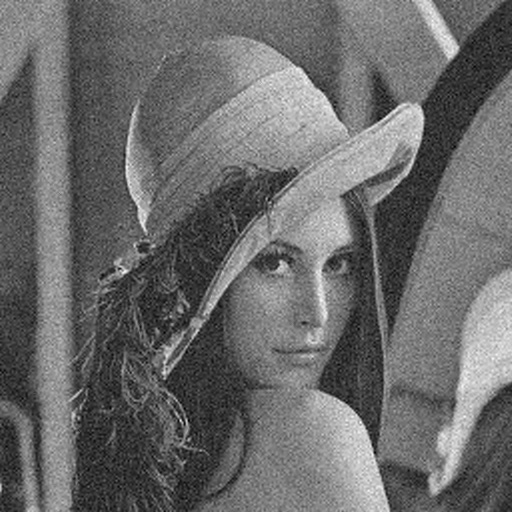
\includegraphics[width=3.5cm]{imgs/Levels/1_normal_soft_sym8_Lenna.jpg}
    \spaced
    \includegraphics[width=3.5cm]{imgs/Levels/2_normal_soft_sym8_Lenna.jpg}
    \\
    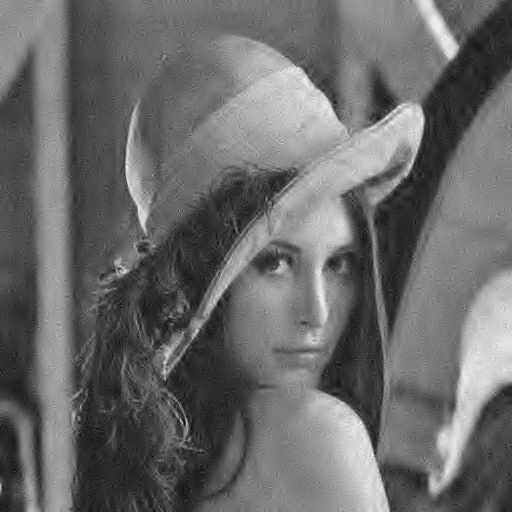
\includegraphics[width=3.5cm]{imgs/Levels/4_normal_soft_sym8_Lenna.jpg}
    \spaced
    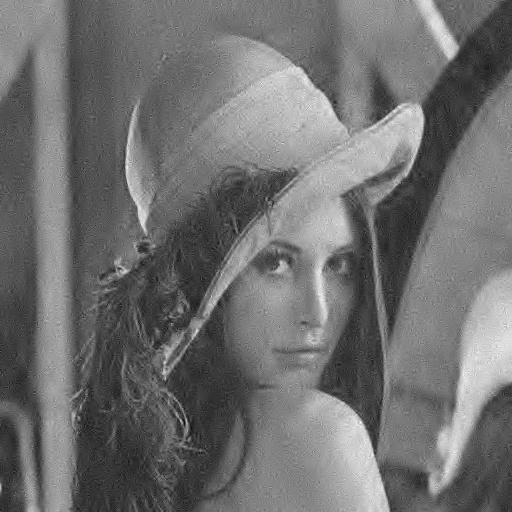
\includegraphics[width=3.5cm]{imgs/Levels/6_normal_soft_sym8_Lenna.jpg}
  
  \end{frame}

  \begin{frame}
    \frametitle{ Comparacion de modos }
    \centering
    \begin{tabular}{lrrr}
      \toprule
      {PSNR} &  noise &   soft &   hard \\
      \midrule
      Lenna &  17.65 &  \bf{27.03} &  21.41 \\
      House &  19.87 &  \bf{25.58} &  20.20 \\
      Wave &  18.63 &  \bf{26.70} &  20.85 \\
      \bottomrule
      \end{tabular}
      \begin{tabular}{lrrr}
        {SSIM} &  noise &   soft &   hard \\
        \midrule
        Lenna &  0.518 &  \bf{0.856} &  0.757 \\
        House &  0.620 &  \bf{0.882} &  0.789 \\
        Wave &  0.586 &  \bf{0.839} &  0.755 \\
        \bottomrule
        \end{tabular}

  \end{frame}

  \begin{frame}
    \frametitle{ Comparacion de modos }
    \centering
    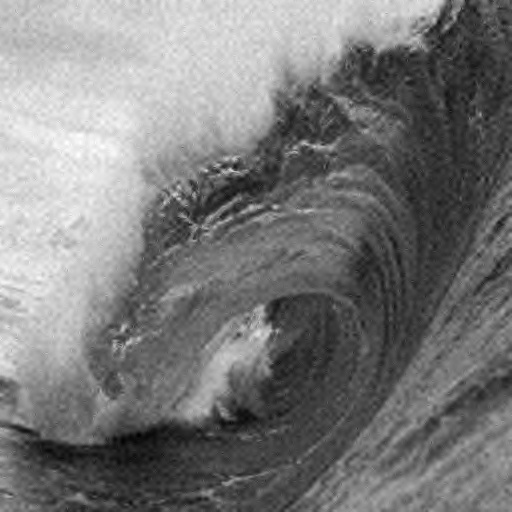
\includegraphics[width=5cm]{imgs/Modes/2_normal_soft_sym8_Wave.jpg}
    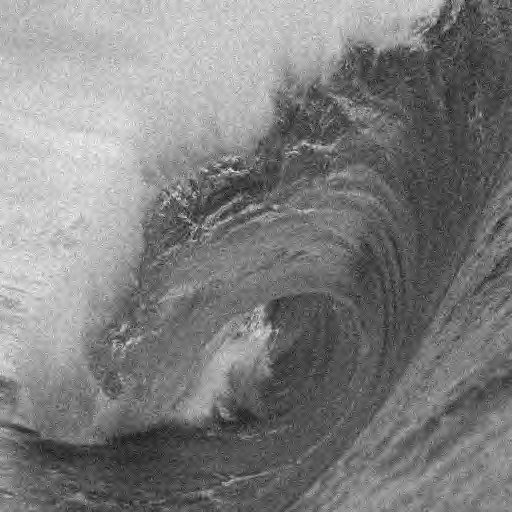
\includegraphics[width=5cm]{imgs/Modes/2_normal_hard_sym8_Wave.jpg}

  \end{frame}

  \begin{frame}
    \frametitle{ Comparacion de umbrales }
    \centering
    \begin{tabular}{lrrrrrr}
      \toprule
      {PSNR} &  noise &  universal &  bayes &  level &  normal &    awt \\
      \midrule
      Lenna &  17.65 &      25.86 &  25.71 &  25.40 &   \bf{27.03} &  25.24 \\
      House &  19.87 &      22.91 &  23.32 &  23.19 &   \bf{25.58} &  23.41 \\
      Wave &  18.63 &      26.74 &  26.70 &  26.86 &   \bf{26.70} &  25.56 \\
      \bottomrule
      \end{tabular}
      \begin{tabular}{lrrrrrr}
        {SSIM} &  noise &  universal &  bayes &  level &  normal &    awt \\
        \midrule
        Lenna &  0.518 &   0.848 &  0.847 &  0.849 &  \bf{0.856} &  0.838 \\
        House &  0.620 &   0.851 &  0.850 &  0.857 &  \bf{0.882} &  0.849 \\
        Wave &  0.586 &   0.830 &  0.829 &  0.833 &  \bf{0.839} &  0.823 \\
        \bottomrule
        \end{tabular}



  \end{frame}

  \begin{frame}
    \frametitle{ Comparacion de umbrales }
  
    \centering
    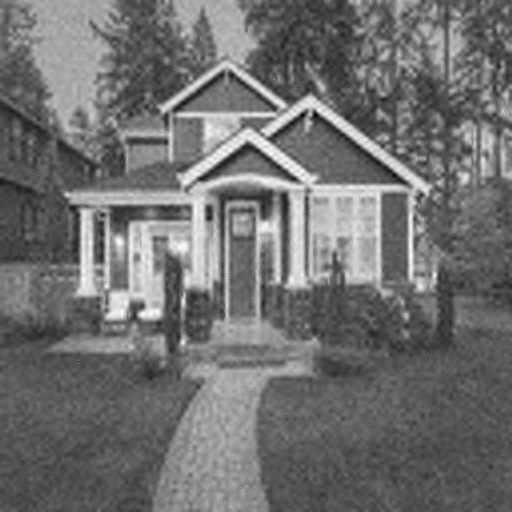
\includegraphics[width=3cm]{imgs/Thresholds/2_awt_soft_sym8_House.jpg}
    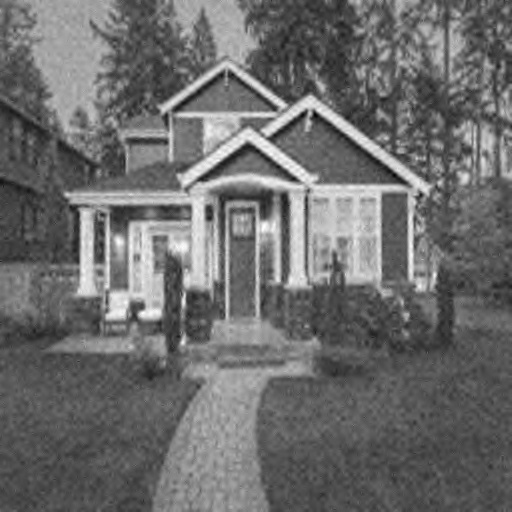
\includegraphics[width=3cm]{imgs/Thresholds/2_normal_soft_sym8_House.jpg}
    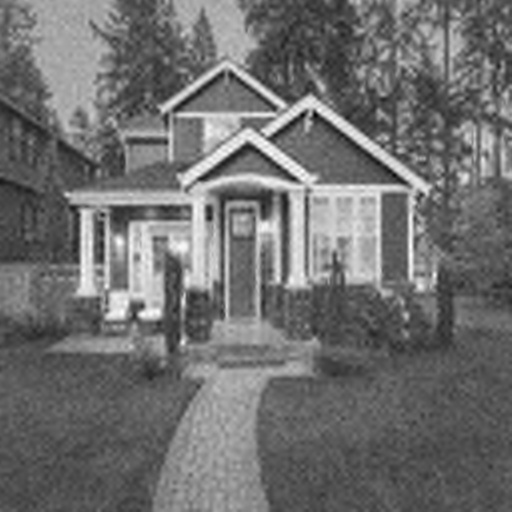
\includegraphics[width=3cm]{imgs/Thresholds/2_universal_soft_sym8_House.jpg}
    \\
    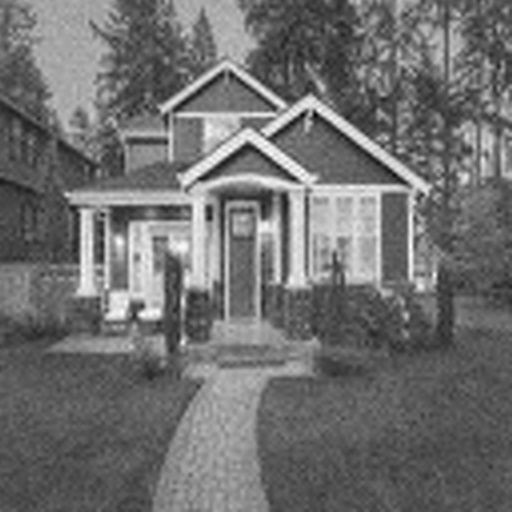
\includegraphics[width=3cm]{imgs/Thresholds/2_bayes_soft_sym8_House.jpg}
    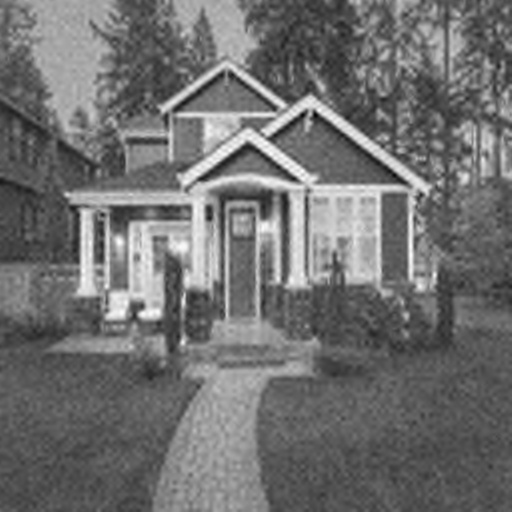
\includegraphics[width=3cm]{imgs/Thresholds/2_level_soft_sym8_House.jpg}
    

  \end{frame}

  \begin{frame}
    \frametitle{Comparacion de la Wavelet madre}
    \centering
    \begin{tabular}{lrrrr}
      \toprule
      {PSNR} &  noise &   haar &    db4 &   sym8 \\
      \midrule
      Lenna &  17.65 &  23.44 & 25.19 &  \bf{27.03} \\
      House &  19.87 &  \bf{26.38} &  24.78 &  25.58 \\
      Wave &  18.63 &  24.67 &  \bf{26.87} &  26.70 \\
      \bottomrule
      \end{tabular}
  
      \begin{tabular}{lrrrr}
        {SSIM} &  noise &   haar &    db4 &   sym8 \\
        \midrule
        Lenna &  0.518 &  0.819 &  0.853 &  \bf{0.856} \\
        House &  0.620 &  0.848 &  0.875 &  \bf{0.882} \\
        Wave &  0.586 &  0.805 &  0.836 &  \bf{0.839} \\
        \bottomrule
        \end{tabular}
  \end{frame}

  \begin{frame}
    \frametitle{Comparacion de la Wavelet madre - db4}
    
    \centering
    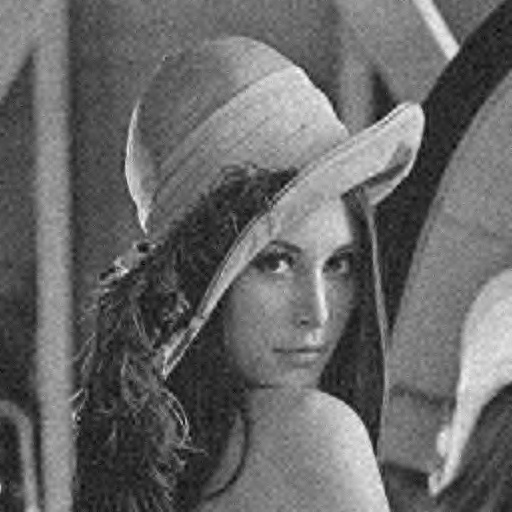
\includegraphics[width=6cm]{imgs/Wavelets/2_normal_soft_db4_Lenna.jpg}
   
  
  \end{frame}

  \begin{frame}
    \frametitle{Comparacion de la Wavelet madre - haar}
    
    \centering
    
    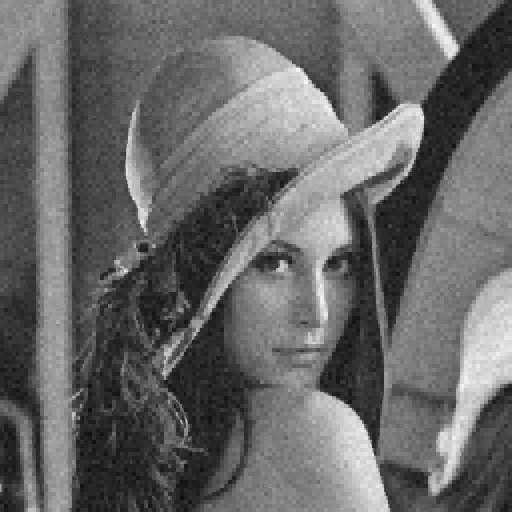
\includegraphics[width=6cm]{imgs/Wavelets/2_normal_soft_haar_Lenna.jpg}
    

  
  \end{frame}

  \begin{frame}
    \frametitle{Comparacion de la Wavelet madre - sym8}
    
    \centering
    
    
    \includegraphics[width=6cm]{imgs/Wavelets/2_normal_soft_sym8_Lenna.jpg}

  
  \end{frame}

  \begin{frame}
    \frametitle{Parametros optimos}
    \centering
    \begin{tabular}{llll}
      \toprule
      level & wavelet & mode & umbral \\
      \midrule 
      2 & sym8 & soft & normal \\
      \bottomrule
    \end{tabular}
  
  \end{frame}

  \subsection{Comparacion de filtros}

  \begin{frame}
    \frametitle{Resultado del filtrado}
  
    
  
  \end{frame}

  \section{Conclusiones}

\end{document}
